\documentclass[11pt]{article}

\usepackage{amsmath}
\usepackage{amsfonts} 
\usepackage{amsthm}
\usepackage{blkarray}
\usepackage{caption}
\usepackage{enumitem} 
\usepackage{mathtools}
\usepackage{tikz}
\usepackage[top=1.5cm,bottom=2cm,left=1.25cm,right=1.75cm,marginparwidth=1.75cm]{geometry}
\setlength{\parindent}{0cm}

\usetikzlibrary{decorations.pathreplacing,decorations.markings}

\newcommand{\R}{\mathbb{R}}
\newcommand\simpleGraph[1]{
  \begin{tikzpicture}[every node/.style={circle,draw}]
    \node (a) at (0,1) {};
    \node (b) at (1,1) {};
    \node (c) at (1,0) {};
    \node (d) at (0,0) {};

    \foreach \from/\to in {#1}
      \draw (\from) -- (\to);
  \end{tikzpicture}\hfil
}
\newcommand\itm[1]{\item[\textbf{#1}]}
\newcommand{\incid}{{-}\!{\bullet}\!{-}}
\newcommand{\n}{\vspace{0.3cm}}

\usetikzlibrary{decorations.pathreplacing,decorations.markings}
\tikzset{
  % style to apply some styles to each segment of a path
  on each segment/.style={
    decorate,
    decoration={
      show path construction,
      moveto code={},
      lineto code={
        \path [#1]
        (\tikzinputsegmentfirst) -- (\tikzinputsegmentlast);
      },
      curveto code={
        \path [#1] (\tikzinputsegmentfirst)
        .. controls
        (\tikzinputsegmentsupporta) and (\tikzinputsegmentsupportb)
        ..
        (\tikzinputsegmentlast);
      },
      closepath code={
        \path [#1]
        (\tikzinputsegmentfirst) -- (\tikzinputsegmentlast);
      },
    },
  },
  % style to add an arrow in the middle of a path
  mid arrow/.style={postaction={decorate,decoration={
        markings,
        mark=at position .5 with {\arrow[#1]{stealth}}
      }}},
}

\def\lc{\left\lceil}   
\def\rc{\right\rceil}
\def\lf{\left\lfloor}   
\def\rf{\right\rfloor}

\newtheorem{theorem}{Theorem}

\title{\vspace{-1.0cm}MATH 5707 Midterm 1}
\author{Fletcher Gornick}
\date{April 5, 2023}

\begin{document}
\maketitle
  \begin{enumerate}
    \item (20 points) \textbf{True} or \textbf{False}.  To receive full credit, assertions which are true must be proven, and those that are false must have a counterexample exhibited.
      \begin{enumerate}[label=(\alph*)]
        \item (5 points) Given a graph \(G\) with connected components \(G_1, \hdots, G_r\), it's chromatic number \(\chi(G)\) satisfies 
          \[\chi(G) = \max \{\chi(G_1), \hdots, \chi(G_r)\}.\]

          \textbf{True.}
          \begin{proof}
            Clearly, \(\chi(G) \geq \max \{\chi(G_1), \hdots, \chi(G_r)\}\), because each connected component is a subgraph. \n

            Let component \(G_i\) achieve this maximum chromatic number.  Since each \(G_j \neq G_i\) has \(\chi(G_j) \leq \chi(G_i)\), we can color each of them with only colors in \(G_i\) (we don't necessarily need to use them all). \n

            Now if we take the union of all these components, we get our original graph \(G\) with \(\chi(G_i)\) colors, and since no components have adjacent vertices, this coloring is proper.  Therefore, we can conclude 
            \[\chi(G) = \chi(G_i) = \max \{\chi(G_1), \hdots, \chi(G_r)\}. \qedhere\]
          \end{proof} \n
          

        \item (5 points) Recall (from lecture or Bondy \& Murty’s Section 3.2) that for every graph \(G\), one can define 2-connected subgraphs \(B_1, \hdots, B_s\) called it's \textit{blocks} or \textit{2-connected components}, whose union is \(G\).  Then the chromatic number \(\chi(G)\) satisfies
          \[\chi(G) = \max \{\chi(B_1), \hdots, \chi(B_s)\}.\]

          \textbf{True.}
          \begin{proof}
            Just like in (a), we can find \(B_i\) achieving maximum chromatic number and color all blocks using the colors in \(B_i\), the only caveat being that for any \(B_j \neq B_i\), there may be a vertex shared between them. \n

            We know there can't be more than one shared vertex between any two blocks, otherwise these two blocks would be two-connected to eachother. \n

            Now assume blocks \(B_j\) and \(B_k\) have been colored but disagree on their shared vertex color.  In this case we can simply rotate colors in one until they agree.  With this, we can now safely take the union and see that 
            \[\chi(G) = \chi(B_i) = \max \{\chi(B_1), \hdots, \chi(B_s)\}. \qedhere\]
          \end{proof} \n
          

        \item (5 points) Given a network digraph \(D = (V,A)\) with distinguished vertices \(s,t \in V\) and edge capacities \(c \colon A \to \R_{\geq 0}\), there is always a \textbf{unique} \(s-t\) flow \(f \colon A \to \R_{\geq 0}\) obeying \(c\) that achieves the maximum value \(\text{val}(f)\).  That is, if both \(f_1, f_2\) obey \(c\) and achieve the maximum flow value \(\text{val}(f_1) = \text{val}(f_2)\), then \(f_1(a) = f_2(a)\) for all \(a \in A\). \n\\
          \textbf{False.}  Take this example from 11.1.1 of the textbook:
          \begin{center}
            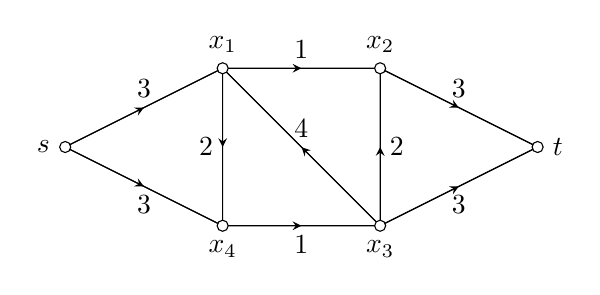
\begin{tikzpicture}
              \tikzset{
                dot/.style = {circle, draw, fill=white, minimum size=#1, inner sep=0pt, outer sep=0pt},
                dot/.default = 4pt
              }
              \node[dot,label=left:{ \(s\)}] (s) at (0,3) {};
              \node[dot,label=right:{ \(t\)}] (t) at (6,3) {};

              \node[dot,label=above:{ \(x_1\)}] (x1) at (2,4) {};
              \node[dot,label=above:{ \(x_2\)}] (x2) at (4,4) {};
              \node[dot,label=below:{ \(x_3\)}] (x3) at (4,2) {};
              \node[dot,label=below:{ \(x_4\)}] (x4) at (2,2) {};

              \path [draw=black, postaction={on each segment={mid arrow=black}}]
                (s) edge node[above] { 3} (x1)
                (s) -- (x1)

                (s) edge node[below] { 3} (x4)
                (s) -- (x4)

                (x1) edge node[above] { 1} (x2)
                (x1) -- (x2)

                (x2) edge node[above] { 3} (t)
                (x2) -- (t)

                (x4) edge node[below] { 1} (x3)
                (x4) -- (x3)

                (x3) edge node[below] { 3} (t)
                (x3) -- (t)

                (x1) edge node[left] { 2} (x4)
                (x1) -- (x4)

                (x3) edge node[right] { 2} (x2)
                (x3) -- (x2)

                (x3) edge node[above] { 4} (x1)
                (x3) -- (x1)
              ;
            \end{tikzpicture}
          \end{center}
          This gives us a bunch of different maximum flows, all with \(\text{val}(f) = 2\).  Here are two:
          \begin{center}
          \resizebox{.75\textwidth}{!} {
            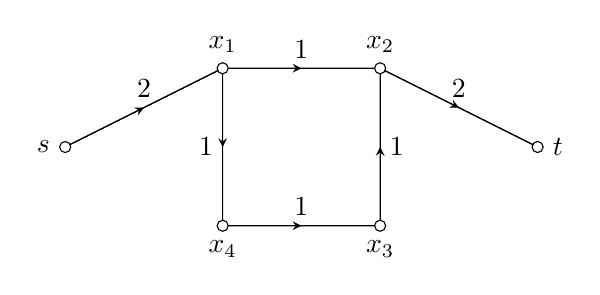
\begin{tikzpicture}
              \tikzset{
                dot/.style = {circle, draw, fill=white, minimum size=#1, inner sep=0pt, outer sep=0pt},
                dot/.default = 4pt
              }
              \node[dot,label=left:{ \(s\)}] (s) at (0,1) {};
              \node[dot,label=right:{ \(t\)}] (t) at (6,1) {};

              \node[dot,label=above:{ \(x_1\)}] (x1) at (2,2) {};
              \node[dot,label=above:{ \(x_2\)}] (x2) at (4,2) {};
              \node[dot,label=below:{ \(x_3\)}] (x3) at (4,0) {};
              \node[dot,label=below:{ \(x_4\)}] (x4) at (2,0) {};

              \path [draw=black, postaction={on each segment={mid arrow=black}}]
                (s) edge node[above] { 2} (x1)
                (s) -- (x1)

                (x1) edge node[left] { 1} (x4)
                (x1) -- (x4)

                (x1) edge node[above] { 1} (x2)
                (x1) -- (x2)

                (x4) edge node[above] { 1} (x3)
                (x4) -- (x3)

                (x3) edge node[right] { 1} (x2)
                (x3) -- (x2)

                (x2) edge node[above] { 2} (t)
                (x2) -- (t)
              ;
            \end{tikzpicture}
            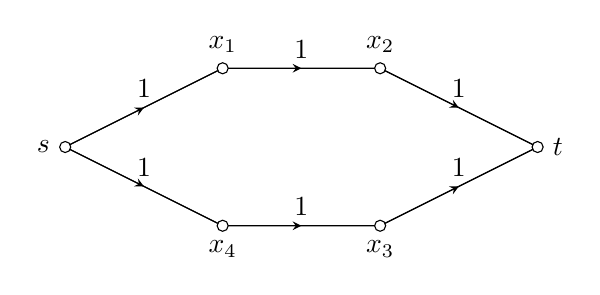
\begin{tikzpicture}
              \tikzset{
                dot/.style = {circle, draw, fill=white, minimum size=#1, inner sep=0pt, outer sep=0pt},
                dot/.default = 4pt
              }
              \node[dot,label=left:{ \(s\)}] (s) at (0,1) {};
              \node[dot,label=right:{ \(t\)}] (t) at (6,1) {};

              \node[dot,label=above:{ \(x_1\)}] (x1) at (2,2) {};
              \node[dot,label=above:{ \(x_2\)}] (x2) at (4,2) {};
              \node[dot,label=below:{ \(x_3\)}] (x3) at (4,0) {};
              \node[dot,label=below:{ \(x_4\)}] (x4) at (2,0) {};

              \path [draw=black, postaction={on each segment={mid arrow=black}}]
                (s) edge node[above] { 1} (x1)
                (s) -- (x1)

                (s) edge node[above] { 1} (x4)
                (s) -- (x4)

                (x4) edge node[above] { 1} (x3)
                (x4) -- (x3)

                (x1) edge node[above] { 1} (x2)
                (x1) -- (x2)

                (x2) edge node[above] { 1} (t)
                (x2) -- (t)

                (x3) edge node[above] { 1} (t)
                (x3) -- (t)
              ;
            \end{tikzpicture}
          }
          \end{center} \n

        \item (5 points) Given the same notation as in part (c), there is always a \textbf{unique} \(s-t\) cut \((S, \bar S)\) (where \(\bar S = V \setminus S\))  that achieves the minimum capacity \(c(S, \bar S) := \sum_{a \in (S, \bar S)} c(a)\).   That is, if both \(S_1,S_2\) contain \(s\) but not \(t\) and achieve the minimum capacity \(c(S_1, \bar S_1) = c(S_2, \bar S_2)\), then \(S_1 = S_2\). \n\\
          \textbf{False.}  Consider this graph below (every cut has capacity 2):
          \begin{center}
            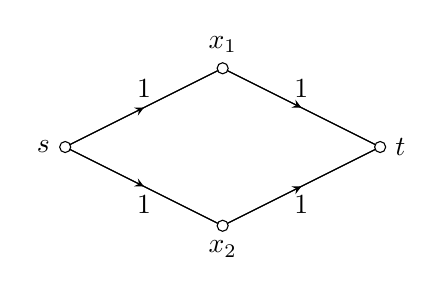
\begin{tikzpicture}
              \tikzset{
                dot/.style = {circle, draw, fill=white, minimum size=#1, inner sep=0pt, outer sep=0pt},
                dot/.default = 4pt
              }
              \node[dot,label=left:{ \(s\)}] (s) at (0,1) {};
              \node[dot,label=right:{ \(t\)}] (t) at (4,1) {};
              \node[dot,label=above:{ \(x_1\)}] (x1) at (2,2) {};
              \node[dot,label=below:{ \(x_2\)}] (x2) at (2,0) {};

              \path [draw=black, postaction={on each segment={mid arrow=black}}]
                (s) edge node[above] {1} (x1)
                (s) -- (x1)
                (x1) edge node[above] {1} (t)
                (x1) -- (t)

                (s) edge node[below] {1} (x2)
                (s) -- (x2)
                (x2) edge node[below] {1} (t)
                (x2) -- (t)
              ;
            \end{tikzpicture}
          \end{center}
          Cuts \(c(\{s\},\{x_1,x_2,t\}) = c(\{s,x_1\},\{x_2,t\}) = c(\{s,x_2\},\{x_1,t\}) = c(\{s,x_1,x_2\},\{t\}) = 2\), so these minimum cuts are not unique.
      \end{enumerate} \n

    \item (20 points) Show that for any simple graph \(G = (V,E)\), one has
      \[|E| \geq \binom{\chi(G)}{2} := \frac{\chi(G)(\chi(G)-1)}{2}.\]
      \begin{proof}
        Let \(f \colon V \to \{1, \hdots, \chi(G)\}\) be our proper \(\chi(G)\)-coloring of \(G\), and let \(V_1, \hdots, V_{\chi(G)}\) be nonempty disjoint subsets of \(V\) such that \(f(V_i) = \{i\}\) for \(1 \leq i \leq \chi(G)\).  I claim, for any \(i,j, \; 1 \leq i < j \leq \chi(G)\), there exists at least one edge between \(V_i\) and \(V_j\). \n

        If there existed components \(V_i,V_j\) with no edge between them, then none of the vertices in \(V_i\) are adjacent to any vertices in \(V_j\), meaning they could all just be given the same color.  So we can reduce the number of colors down to \(\chi(G)-1\) which is a contradiction. \n

        Since each component is connected to every other component, and there are \(\chi(G)\) components, we get the following inequality:
        \[|E| \geq (\chi(G)-1) + (\chi(G)-2) + \hdots + 1 = \sum_{i=1}^{\chi(G)-1} i = \frac{\chi(G)(\chi(G)-1)}{2} = \binom{\chi(G)}{2}. \qedhere\]
      \end{proof}
      

    \item (20 points) Given a simple graph \(G = (V,E)\), a subset \(V' \subseteq V\) is called an \textit{independent} or \textit{stable} set of vertices if there are no edges \(xy \in E\) with \(x,y \in V'\). Let
      \[\alpha(G) := \max \{|V'| \colon V' \subseteq V \text{ is an independent subset}\}.\]
      Prove the following inequalities.  When proving any of the later parts, you may assume the inequalities from any of the previous parts, whether or not you were able to prove them.
      \begin{enumerate}[label=(\alph*)]
        \item (5 points) Show the complement graph \(\bar G\) has \(\chi(\bar G) \geq \alpha(G)\).
          \begin{proof}
            Suppose \(V' \subseteq V\) is the maximum stable set of \(G\) (\(|V'| = \alpha(G)\)), so for all \(x,y \in V'\), \(xy \not\in E(G)\).  This means in the complement \(\bar G\), for all \(x,y \in V'\), \(xy \in E(\bar G)\). \n

            Let \(G'\) be a subgraph of \(\bar G\) with vertex set \(V'\).  Since \(xy \in E(G')\) for all \(x,y \in V(G')\), we have that \(G' = K_{|V'|}\), so \(\chi(G') = |V'| = \alpha(G)\).  Finally, since \(G' \subseteq \bar G\), we can conclude that 
            \[\chi(\bar G) \geq \chi(G') = \alpha(G). \qedhere\]
          \end{proof}
          

        \item (5 points) Show that \(\chi(G) \cdot \alpha(G) \geq |V|\).
          \begin{proof}
            If we decompose \(G\) into disjoint sets \(V = V_1 \cup V_2 \cup \hdots \cup V_{\chi(G)}\) corresponding to a proper coloring, then we know that each \(V_i\) is a stable set. If \(V_i\) weren't a stable set, and there existed vertices \(u,v \in V_i\) with \(uv \in E(G)\), then we wouldn't be allowed to assign \(u,v\) the same color in our proper coloring, hence \(V_i\) cannot contain such vertices and must be a stable set. \n

            Since each of our disjoint subsets are stable, and \(\alpha(G)\) is the maximum size of a stable set in \(V\), we know \(|V_i| \leq \alpha(G)\) for all \(i, \; 1 \leq i \leq \chi(G)\).  This gives us the following relation:
            \[|V| = \sum_{i=1}^{\chi(G)} |V_i| \leq \sum_{i=1}^{\chi(G)} \alpha(G) = \chi(G) \cdot \alpha(G). \qedhere\]
          \end{proof}
          

        \item (5 points) Show that \(\chi(G) \cdot \chi(\bar G) \geq |V|\).
          \begin{proof}
            This follows directly from (a) and (b): \(\chi(G) \cdot \chi(\bar G) \geq \chi(G) \cdot \alpha(G) \geq |V|\).
          \end{proof}
          

        \item (5 points) Show that \(\chi(G) + \chi(\bar G) \geq 2 \sqrt{|V|}\).
          \begin{proof}
            The arithmetic-geometric mean inequality states that for any two nonnegative integers \(x,y\):
            \[x + y \;\geq\; 2 \sqrt{xy}.\]
            Using this in conjunction with our result from (c) yields the desired inequality:
            \[\chi(G) + \chi(\bar G) \;\geq\; 2 \sqrt{\chi(G) \cdot \chi(\bar G)} \;\geq\; 2 \sqrt{|V|}. \qedhere\]
          \end{proof}
          
      \end{enumerate} \n

    \item (20 points) Let \(G = (X \cup Y, E)\) be a bipartite graph, and assume that there are integers \(d_X, d_Y \geq 1\) such that every \(x \in X\) has \(d_G(x) = d_X\) and every \(y \in Y\) has \(d_G(y) = d_Y\).
      \begin{enumerate}
        \item (10 points) Prove that \(d_X / d_Y = |Y|/|X|\).
          \begin{proof}
            First, note that in a bipartite graph \(G = (X \cup Y, E)\), \(\sum_{x \in X} d_G(x) = \sum_{y \in Y} d_G(y) = |E|\), this is because (via the argument given in our first lecture):
            \[\sum_{x \in X} d_G(x) = (\text{\# of edges incident to } X) = |E| = (\text{\# of edges incident to } Y) = \sum_{y \in Y} d_G(y).\]
            Using this, we get the following equalities:
            \begin{align*}
              |X| \cdot d_X = \sum_{x \in X} d_X = \sum_{x \in X} d_G(x)  &= \sum_{y \in Y} d_G(y) = \sum_{y \in Y} d_Y = |Y| \cdot d_Y \\
              \iff d_X / d_Y &= |Y| / |X|. \qedhere
            \end{align*}
          \end{proof}
          

        \item (10 points) Prove that if \(d_X \geq d_Y\) then there exists a matching \(M \subseteq E\) that matches every \(x \in X\).
          \begin{proof}
            For a set \(S\) of vertices in \(G\), the \textit{neighbor set} \(N(S)\) is defined to be the set of vertices adjacent to the vertices in \(S\).  We begin by showing for all subsets \(X' \subseteq X\), \(|X'| \leq |N(X')|\). \n

            Suppose, to the contrary, there exists \(X' \subseteq X\) such that \(|X'| \geq |N(X')|\).  Since \(G\) is bipartite, we know \(N(X') \subseteq Y\).  Every edge coming out of \(X'\) must go into \(N(X')\), otherwise our neighbor set doesn't contain all neighboring edges.  Also, each vertex \(x \in X\) has degree \(d_G(x) = d_X\), similarly, \(d_G(y) = d_Y\) for all \(y \in N(X')\). \n

            The degree sum of \(N(X')\) must be at least the degree sum of \(X'\) (all edges in \(X'\) are in \(N(X')\)), potentially more if there are vericies \(x \in X \setminus X'\) adjacent to some \(y \in N(X')\), but this tells us:
            \[d_Y \cdot |N(X')| = \sum_{y \in N(X')} d_G(y) \geq \sum_{x \in X'} d_G(x) = d_X \cdot |X'|.\]
            But \(d_Y \leq d_X\) and \(|N(X')| < |X'|\), the above inequality clearly cannot be possible, so we conclude that for all \(X' \subseteq X\), \(|X'| \leq |N(X')|\).  Finally, applying theorem 5.2, since  \(|X'| \leq |N(X')|\) for all  \(X' \subseteq X\), \(G\) must contain a matching that saturates every \(x \in X\).
          \end{proof} \n
          

      \end{enumerate}

    \item (20 points) Let \(G = (X \cup Y, E)\) be a bipartite graph which is \(d\)-regular (all vertices have degree \(d\)) with \(d \geq 2\).  If \(G\) is connected, prove that \(G\) has no cut-edge, that is \(G - e\) is connected for every \(e \in E\).
  \end{enumerate}
\end{document}
